\documentclass{standalone}
\usepackage{tikz}
\usetikzlibrary{patterns, positioning}

\begin{document}
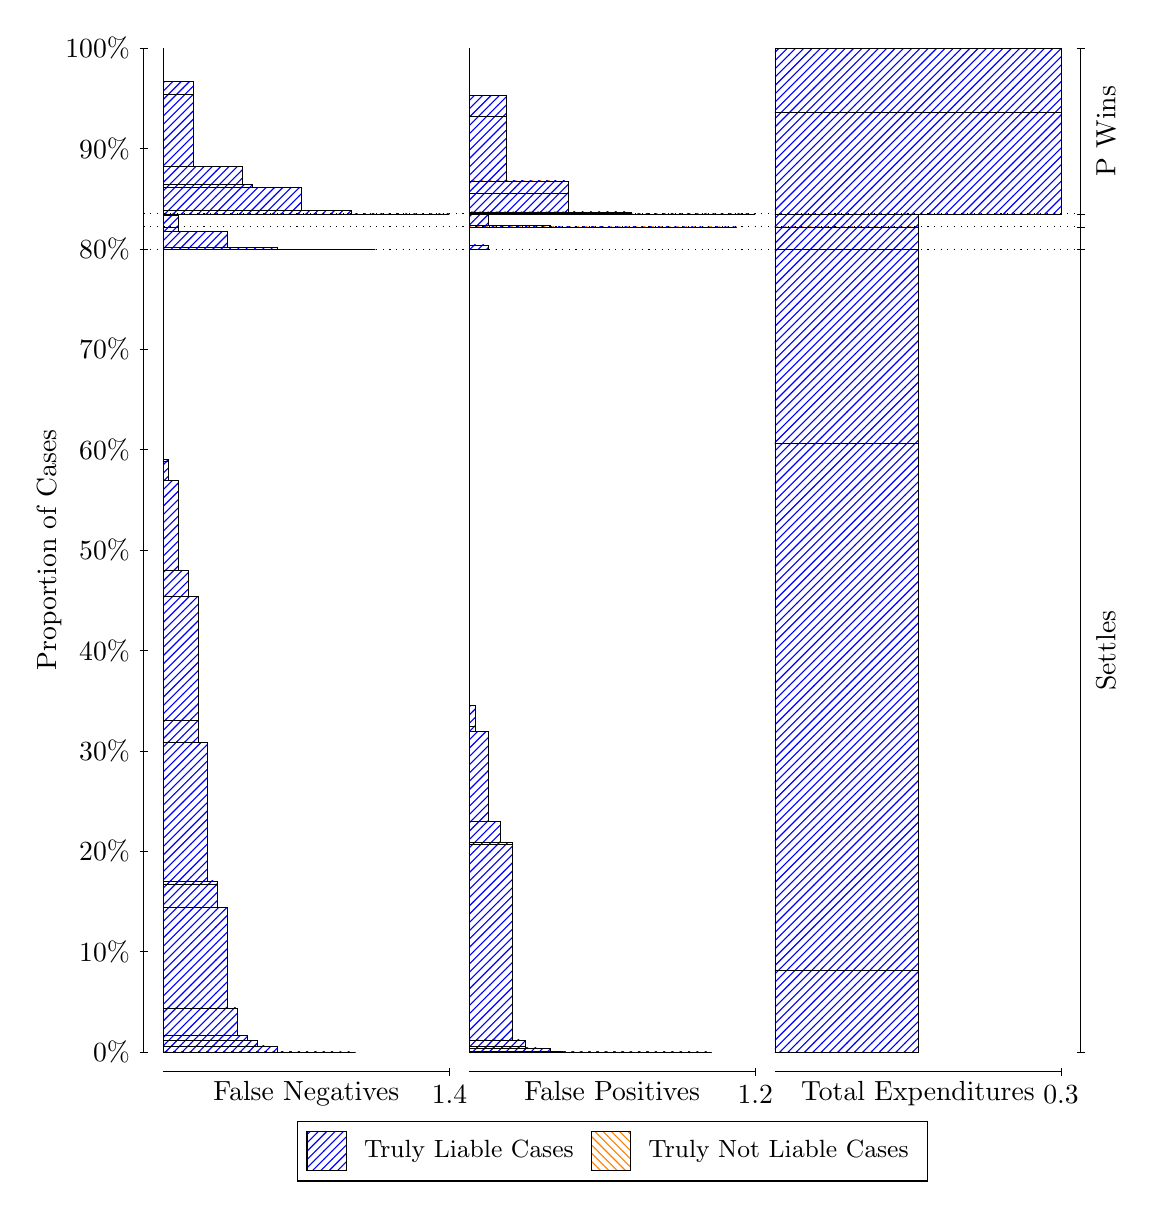
\begin{tikzpicture}
\draw[black, very thin] (1.5,1.75) -- (1.5,14.5);
\node[rotate=90, anchor=center] at (0.3, 8.125) {Proportion of Cases};
\draw[black, very thin] (1.45,1.75) -- (1.55,1.75);
\node[anchor=east] at (1.45, 1.75) {0\%};
\draw[black, very thin] (1.45,3.025) -- (1.55,3.025);
\node[anchor=east] at (1.45, 3.025) {10\%};
\draw[black, very thin] (1.45,4.3) -- (1.55,4.3);
\node[anchor=east] at (1.45, 4.3) {20\%};
\draw[black, very thin] (1.45,5.575) -- (1.55,5.575);
\node[anchor=east] at (1.45, 5.575) {30\%};
\draw[black, very thin] (1.45,6.85) -- (1.55,6.85);
\node[anchor=east] at (1.45, 6.85) {40\%};
\draw[black, very thin] (1.45,8.125) -- (1.55,8.125);
\node[anchor=east] at (1.45, 8.125) {50\%};
\draw[black, very thin] (1.45,9.4) -- (1.55,9.4);
\node[anchor=east] at (1.45, 9.4) {60\%};
\draw[black, very thin] (1.45,10.675) -- (1.55,10.675);
\node[anchor=east] at (1.45, 10.675) {70\%};
\draw[black, very thin] (1.45,11.95) -- (1.55,11.95);
\node[anchor=east] at (1.45, 11.95) {80\%};
\draw[black, very thin] (1.45,13.225) -- (1.55,13.225);
\node[anchor=east] at (1.45, 13.225) {90\%};
\draw[black, very thin] (1.45,14.5) -- (1.55,14.5);
\node[anchor=east] at (1.45, 14.5) {100\%};

\draw[black, very thin] (13.4,1.75) -- (13.4,14.5);
\draw[black, very thin] (13.35,1.75) -- (13.45,1.75);
\node[anchor=west] at (13.35, 1.75) {};
\draw[black, very thin] (13.35,11.941) -- (13.45,11.941);
\node[anchor=west] at (13.35, 11.941) {};
\draw[black, very thin] (13.35,12.228) -- (13.45,12.228);
\node[anchor=west] at (13.35, 12.228) {};
\draw[black, very thin] (13.35,12.395) -- (13.45,12.395);
\node[anchor=west] at (13.35, 12.395) {};
\draw[black, very thin] (13.35,14.5) -- (13.45,14.5);
\node[anchor=west] at (13.35, 14.5) {};

\draw[black, very thin, pattern color=blue, pattern=north east lines] (1.75,1.75) rectangle (4.1931,1.75);
\draw[black, very thin, pattern color=blue, pattern=north east lines] (1.75,1.75) rectangle (3.9425,1.75);
\draw[black, very thin, pattern color=blue, pattern=north east lines] (1.75,1.75) rectangle (3.692,1.75);
\draw[black, very thin, pattern color=blue, pattern=north east lines] (1.75,1.75) rectangle (3.5667,1.75);
\draw[black, very thin, pattern color=blue, pattern=north east lines] (1.75,1.75) rectangle (3.4414,1.7502);
\draw[black, very thin, pattern color=blue, pattern=north east lines] (1.75,1.7502) rectangle (3.3161,1.7503);
\draw[black, very thin, pattern color=blue, pattern=north east lines] (1.75,1.7503) rectangle (3.1908,1.8219);
\draw[black, very thin, pattern color=blue, pattern=north east lines] (1.75,1.8219) rectangle (3.0655,1.8276);
\draw[black, very thin, pattern color=blue, pattern=north east lines] (1.75,1.8276) rectangle (2.9402,1.898);
\draw[black, very thin, pattern color=blue, pattern=north east lines] (1.75,1.898) rectangle (2.8149,1.8982);
\draw[black, very thin, pattern color=blue, pattern=north east lines] (1.75,1.8982) rectangle (2.8149,1.965);
\draw[black, very thin, pattern color=blue, pattern=north east lines] (1.75,1.965) rectangle (2.6897,2.3104);
\draw[black, very thin, pattern color=blue, pattern=north east lines] (1.75,2.3104) rectangle (2.5644,3.5857);
\draw[black, very thin, pattern color=blue, pattern=north east lines] (1.75,3.5857) rectangle (2.4391,3.8859);
\draw[black, very thin, pattern color=blue, pattern=north east lines] (1.75,3.8859) rectangle (2.4391,3.9216);
\draw[black, very thin, pattern color=blue, pattern=north east lines] (1.75,3.9216) rectangle (2.3138,5.6813);
\draw[black, very thin, pattern color=blue, pattern=north east lines] (1.75,5.6813) rectangle (2.1885,5.6869);
\draw[black, very thin, pattern color=blue, pattern=north east lines] (1.75,5.6869) rectangle (2.1885,5.9573);
\draw[black, very thin, pattern color=blue, pattern=north east lines] (1.75,5.9573) rectangle (2.1885,7.5405);
\draw[black, very thin, pattern color=blue, pattern=north east lines] (1.75,7.5405) rectangle (2.0632,7.8702);
\draw[black, very thin, pattern color=blue, pattern=north east lines] (1.75,7.8702) rectangle (1.9379,9.008);
\draw[black, very thin, pattern color=blue, pattern=north east lines] (1.75,9.008) rectangle (1.8126,9.2514);
\draw[black, very thin, pattern color=blue, pattern=north east lines] (1.75,9.2514) rectangle (1.8126,9.2768);
\draw[black, very thin, pattern color=orange, pattern=north west lines] (1.75,9.2768) rectangle (1.75,9.2768);
\draw[black, very thin, pattern color=blue, pattern=north east lines] (1.75,9.2768) rectangle (1.75,11.941);
\draw[black, very thin, pattern color=blue, pattern=north east lines] (1.75,11.941) rectangle (4.4437,11.941);
\draw[black, very thin, pattern color=blue, pattern=north east lines] (1.75,11.941) rectangle (3.8172,11.941);
\draw[black, very thin, pattern color=blue, pattern=north east lines] (1.75,11.941) rectangle (3.1908,11.971);
\draw[black, very thin, pattern color=blue, pattern=north east lines] (1.75,11.971) rectangle (2.5644,12.17);
\draw[black, very thin, pattern color=blue, pattern=north east lines] (1.75,12.17) rectangle (1.9379,12.228);
\draw[black, very thin, pattern color=orange, pattern=north west lines] (1.75,12.228) rectangle (1.75,12.228);
\draw[black, very thin, pattern color=blue, pattern=north east lines] (1.75,12.228) rectangle (1.9379,12.375);
\draw[black, very thin, pattern color=orange, pattern=north west lines] (1.75,12.375) rectangle (1.75,12.375);
\draw[black, very thin, pattern color=blue, pattern=north east lines] (1.75,12.375) rectangle (1.75,12.395);
\draw[black, very thin, pattern color=blue, pattern=north east lines] (1.75,12.395) rectangle (5.3833,12.395);
\draw[black, very thin, pattern color=blue, pattern=north east lines] (1.75,12.395) rectangle (4.7569,12.395);
\draw[black, very thin, pattern color=blue, pattern=north east lines] (1.75,12.395) rectangle (4.1305,12.437);
\draw[black, very thin, pattern color=blue, pattern=north east lines] (1.75,12.437) rectangle (4.0052,12.437);
\draw[black, very thin, pattern color=blue, pattern=north east lines] (1.75,12.437) rectangle (3.504,12.733);
\draw[black, very thin, pattern color=blue, pattern=north east lines] (1.75,12.733) rectangle (3.3787,12.733);
\draw[black, very thin, pattern color=blue, pattern=north east lines] (1.75,12.733) rectangle (2.8776,12.769);
\draw[black, very thin, pattern color=blue, pattern=north east lines] (1.75,12.769) rectangle (2.7523,12.994);
\draw[black, very thin, pattern color=blue, pattern=north east lines] (1.75,12.994) rectangle (2.2511,12.994);
\draw[black, very thin, pattern color=blue, pattern=north east lines] (1.75,12.994) rectangle (2.1259,13.908);
\draw[black, very thin, pattern color=blue, pattern=north east lines] (1.75,13.908) rectangle (2.1259,14.081);
\draw[black, very thin, pattern color=orange, pattern=north west lines] (1.75,14.081) rectangle (1.75,14.081);
\draw[black, very thin, pattern color=blue, pattern=north east lines] (1.75,14.081) rectangle (1.75,14.5);
\draw[black, very thin, pattern color=orange, pattern=north west lines] (5.6333,1.75) rectangle (8.7138,1.75);
\draw[black, very thin, pattern color=blue, pattern=north east lines] (5.6333,1.75) rectangle (8.7138,1.75);
\draw[black, very thin, pattern color=orange, pattern=north west lines] (5.6333,1.75) rectangle (8.3978,1.75);
\draw[black, very thin, pattern color=blue, pattern=north east lines] (5.6333,1.75) rectangle (8.3978,1.75);
\draw[black, very thin, pattern color=orange, pattern=north west lines] (5.6333,1.75) rectangle (8.0819,1.75);
\draw[black, very thin, pattern color=blue, pattern=north east lines] (5.6333,1.75) rectangle (8.0819,1.75);
\draw[black, very thin, pattern color=blue, pattern=north east lines] (5.6333,1.75) rectangle (7.9239,1.75);
\draw[black, very thin, pattern color=orange, pattern=north west lines] (5.6333,1.75) rectangle (7.7659,1.75);
\draw[black, very thin, pattern color=blue, pattern=north east lines] (5.6333,1.75) rectangle (7.7659,1.75);
\draw[black, very thin, pattern color=blue, pattern=north east lines] (5.6333,1.75) rectangle (7.608,1.75);
\draw[black, very thin, pattern color=orange, pattern=north west lines] (5.6333,1.75) rectangle (7.45,1.75);
\draw[black, very thin, pattern color=blue, pattern=north east lines] (5.6333,1.75) rectangle (7.45,1.75);
\draw[black, very thin, pattern color=blue, pattern=north east lines] (5.6333,1.75) rectangle (7.292,1.75);
\draw[black, very thin, pattern color=orange, pattern=north west lines] (5.6333,1.75) rectangle (7.1341,1.75);
\draw[black, very thin, pattern color=blue, pattern=north east lines] (5.6333,1.75) rectangle (7.1341,1.75);
\draw[black, very thin, pattern color=orange, pattern=north west lines] (5.6333,1.75) rectangle (7.1341,1.75);
\draw[black, very thin, pattern color=blue, pattern=north east lines] (5.6333,1.75) rectangle (7.1341,1.7501);
\draw[black, very thin, pattern color=blue, pattern=north east lines] (5.6333,1.7501) rectangle (6.9761,1.7502);
\draw[black, very thin, pattern color=orange, pattern=north west lines] (5.6333,1.7502) rectangle (6.8181,1.7502);
\draw[black, very thin, pattern color=blue, pattern=north east lines] (5.6333,1.7502) rectangle (6.8181,1.7533);
\draw[black, very thin, pattern color=blue, pattern=north east lines] (5.6333,1.7533) rectangle (6.6601,1.7987);
\draw[black, very thin, pattern color=orange, pattern=north west lines] (5.6333,1.7987) rectangle (6.5022,1.7987);
\draw[black, very thin, pattern color=blue, pattern=north east lines] (5.6333,1.7987) rectangle (6.5022,1.7996);
\draw[black, very thin, pattern color=blue, pattern=north east lines] (5.6333,1.7996) rectangle (6.5022,1.8025);
\draw[black, very thin, pattern color=blue, pattern=north east lines] (5.6333,1.8025) rectangle (6.3442,1.8203);
\draw[black, very thin, pattern color=blue, pattern=north east lines] (5.6333,1.8203) rectangle (6.3442,1.9033);
\draw[black, very thin, pattern color=orange, pattern=north west lines] (5.6333,1.9033) rectangle (6.1862,1.9033);
\draw[black, very thin, pattern color=blue, pattern=north east lines] (5.6333,1.9033) rectangle (6.1862,4.3867);
\draw[black, very thin, pattern color=blue, pattern=north east lines] (5.6333,4.3867) rectangle (6.1862,4.4138);
\draw[black, very thin, pattern color=blue, pattern=north east lines] (5.6333,4.4138) rectangle (6.0283,4.6825);
\draw[black, very thin, pattern color=blue, pattern=north east lines] (5.6333,4.6825) rectangle (5.8703,5.8204);
\draw[black, very thin, pattern color=blue, pattern=north east lines] (5.6333,5.8204) rectangle (5.7123,5.8886);
\draw[black, very thin, pattern color=blue, pattern=north east lines] (5.6333,5.8886) rectangle (5.7123,6.15);
\draw[black, very thin, pattern color=blue, pattern=north east lines] (5.6333,6.15) rectangle (5.6333,11.941);
\draw[black, very thin, pattern color=orange, pattern=north west lines] (5.6333,11.941) rectangle (5.8703,11.941);
\draw[black, very thin, pattern color=blue, pattern=north east lines] (5.6333,11.941) rectangle (5.8703,11.999);
\draw[black, very thin, pattern color=blue, pattern=north east lines] (5.6333,11.999) rectangle (5.6333,12.228);
\draw[black, very thin, pattern color=orange, pattern=north west lines] (5.6333,12.228) rectangle (9.0297,12.228);
\draw[black, very thin, pattern color=blue, pattern=north east lines] (5.6333,12.228) rectangle (9.0297,12.228);
\draw[black, very thin, pattern color=blue, pattern=north east lines] (5.6333,12.228) rectangle (8.2399,12.228);
\draw[black, very thin, pattern color=blue, pattern=north east lines] (5.6333,12.228) rectangle (7.45,12.228);
\draw[black, very thin, pattern color=blue, pattern=north east lines] (5.6333,12.228) rectangle (6.6601,12.247);
\draw[black, very thin, pattern color=blue, pattern=north east lines] (5.6333,12.247) rectangle (5.8703,12.395);
\draw[black, very thin, pattern color=orange, pattern=north west lines] (5.6333,12.395) rectangle (9.2667,12.395);
\draw[black, very thin, pattern color=blue, pattern=north east lines] (5.6333,12.395) rectangle (9.2667,12.395);
\draw[black, very thin, pattern color=orange, pattern=north west lines] (5.6333,12.395) rectangle (8.4768,12.395);
\draw[black, very thin, pattern color=blue, pattern=north east lines] (5.6333,12.395) rectangle (8.4768,12.395);
\draw[black, very thin, pattern color=blue, pattern=north east lines] (5.6333,12.395) rectangle (8.4768,12.395);
\draw[black, very thin, pattern color=orange, pattern=north west lines] (5.6333,12.395) rectangle (7.687,12.395);
\draw[black, very thin, pattern color=blue, pattern=north east lines] (5.6333,12.395) rectangle (7.687,12.403);
\draw[black, very thin, pattern color=blue, pattern=north east lines] (5.6333,12.403) rectangle (7.687,12.418);
\draw[black, very thin, pattern color=orange, pattern=north west lines] (5.6333,12.418) rectangle (6.8971,12.418);
\draw[black, very thin, pattern color=blue, pattern=north east lines] (5.6333,12.418) rectangle (6.8971,12.655);
\draw[black, very thin, pattern color=blue, pattern=north east lines] (5.6333,12.655) rectangle (6.8971,12.814);
\draw[black, very thin, pattern color=orange, pattern=north west lines] (5.6333,12.814) rectangle (6.7391,12.814);
\draw[black, very thin, pattern color=blue, pattern=north east lines] (5.6333,12.814) rectangle (6.7391,12.814);
\draw[black, very thin, pattern color=blue, pattern=north east lines] (5.6333,12.814) rectangle (6.1072,13.631);
\draw[black, very thin, pattern color=blue, pattern=north east lines] (5.6333,13.631) rectangle (6.1072,13.901);
\draw[black, very thin, pattern color=orange, pattern=north west lines] (5.6333,13.901) rectangle (5.9493,13.901);
\draw[black, very thin, pattern color=blue, pattern=north east lines] (5.6333,13.901) rectangle (5.9493,13.901);
\draw[black, very thin, pattern color=blue, pattern=north east lines] (5.6333,13.901) rectangle (5.9493,13.901);
\draw[black, very thin, pattern color=orange, pattern=north west lines] (5.6333,13.901) rectangle (5.6333,13.901);
\draw[black, very thin, pattern color=blue, pattern=north east lines] (5.6333,13.901) rectangle (5.6333,14.5);
\draw[black, very thin, pattern color=orange, pattern=north west lines] (9.5167,1.75) rectangle (11.333,1.75);
\draw[black, very thin, pattern color=blue, pattern=north east lines] (9.5167,1.75) rectangle (11.333,2.7872);
\draw[black, very thin, pattern color=orange, pattern=north west lines] (9.5167,2.7872) rectangle (11.333,2.7872);
\draw[black, very thin, pattern color=blue, pattern=north east lines] (9.5167,2.7872) rectangle (11.333,9.4815);
\draw[black, very thin, pattern color=orange, pattern=north west lines] (9.5167,9.4815) rectangle (11.333,9.4815);
\draw[black, very thin, pattern color=blue, pattern=north east lines] (9.5167,9.4815) rectangle (11.333,11.941);
\draw[black, very thin, pattern color=orange, pattern=north west lines] (9.5167,11.941) rectangle (11.333,11.941);
\draw[black, very thin, pattern color=blue, pattern=north east lines] (9.5167,11.941) rectangle (11.333,12.228);
\draw[black, very thin, pattern color=orange, pattern=north west lines] (9.5167,12.228) rectangle (11.333,12.228);
\draw[black, very thin, pattern color=blue, pattern=north east lines] (9.5167,12.228) rectangle (11.333,12.395);
\draw[black, very thin, pattern color=orange, pattern=north west lines] (9.5167,12.395) rectangle (13.15,12.395);
\draw[black, very thin, pattern color=blue, pattern=north east lines] (9.5167,12.395) rectangle (13.15,13.682);
\draw[black, very thin, pattern color=orange, pattern=north west lines] (9.5167,13.682) rectangle (13.15,13.682);
\draw[black, very thin, pattern color=blue, pattern=north east lines] (9.5167,13.682) rectangle (13.15,14.5);
\draw[black, dotted] (1.5,11.941) -- (13.4,11.941);
\draw[black, dotted] (1.5,12.228) -- (13.4,12.228);
\draw[black, dotted] (1.5,12.395) -- (13.4,12.395);
\draw[black, very thin] (1.75,1.5) -- (5.3833,1.5);
\node[anchor=north] at (3.5667, 1.5) {False Negatives};
\draw[black, very thin] (5.3833,1.45) -- (5.3833,1.55);
\node[anchor=north] at (5.3833, 1.45) {1.4};

\draw[black, very thin] (5.6333,1.5) -- (9.2667,1.5);
\node[anchor=north] at (7.45, 1.5) {False Positives};
\draw[black, very thin] (9.2667,1.45) -- (9.2667,1.55);
\node[anchor=north] at (9.2667, 1.45) {1.2};

\draw[black, very thin] (9.5167,1.5) -- (13.15,1.5);
\node[anchor=north] at (11.333, 1.5) {Total Expenditures};
\draw[black, very thin] (13.15,1.45) -- (13.15,1.55);
\node[anchor=north] at (13.15, 1.45) {0.3};

\node[black, centered, rotate=90] at (13.72, 6.8453) {Settles};


\node[black, centered, rotate=90] at (13.72, 13.447) {P Wins};

\draw (7.449999999999999,1.5) node[draw=none] (baseCoordinate) {};
\begin{scope}[align=center]
        \matrix[scale=0.5, draw=black, below=0.5cm of baseCoordinate, nodes={draw}, column sep=0.1cm]{
            \node[rectangle, draw, minimum width=0.5cm, minimum height=0.5cm, pattern=north east lines, pattern color=blue] {}; &
            \node[draw=none, font=\small] (B) {Truly Liable Cases}; &
            \node[rectangle, draw, minimum width=0.5cm, minimum height=0.5cm, pattern=north west lines, pattern color=orange] {}; &
            \node[draw=none, font=\small] (B) {Truly Not Liable Cases}; \\
            };
\end{scope}

\end{tikzpicture}
\end{document}